\chapter{Testing}

This section documents the tests used to ensure that the implementation of Liquid State Machine is functional, and to highlight certain properties of both the implementation and the network model itself.

\section{Neuron model}

There exists several neural models that can be used for a Liquid State Machine, or a Spiking Neural Network. The selected model is the Leaky-Integrate-and-Fire model \ref{sec:leaky}, as it is simple, not computationally heavy, and expressive enough for this project.

In order to test this model, a baseline set of parameters must first be selected. The baseline parameters can be found in table \ref{tab:model1}. For these parameters, the model behaves as can be seen in figure \ref{fig:model1} which is clearly a smooth membrane potential curve followed by a spike as the potential reaches the spiking threshold. In figure \ref{fig:model2}, the parameters have been changed to allow a random input between zero and one, thus illustrating how a neuron would act when it's input is affected by several synapses that fire independent of each other. It is clear from these two images, as the neuron fires in exactly the same timestep, that the mean input is relevant, even if the input is not consistent.

\begin{figure}
    \centering
    \begin{subfigure}[b]{0.3\textwidth}
        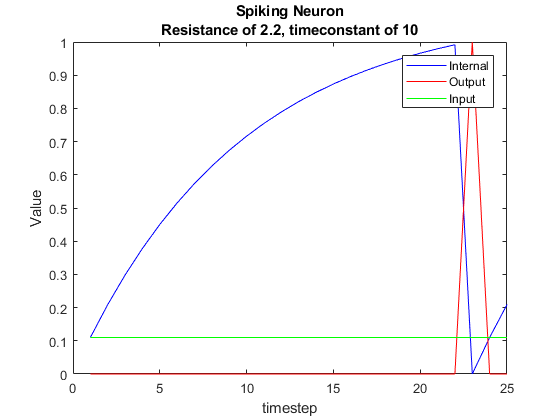
\includegraphics[width=\textwidth]{Images/slow.png}
        \caption{The neuron model using the baseline parameters and constant input of 0.5.}
        \label{fig:implementation_test}
    \end{subfigure}
    \begin{subfigure}[b]{0.3\textwidth}
        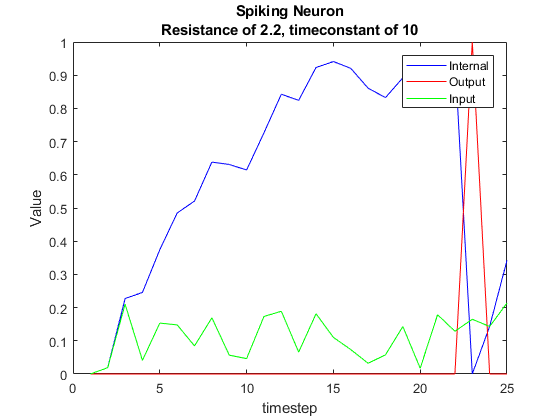
\includegraphics[width=\textwidth]{Images/randomInput.png}
        \caption{The neuron model using the baseline parameters and random input with a mean of 0.5.}
        \label{fig:implementation_test}
    \end{subfigure}
    \begin{subfigure}[b]{0.3\textwidth}
        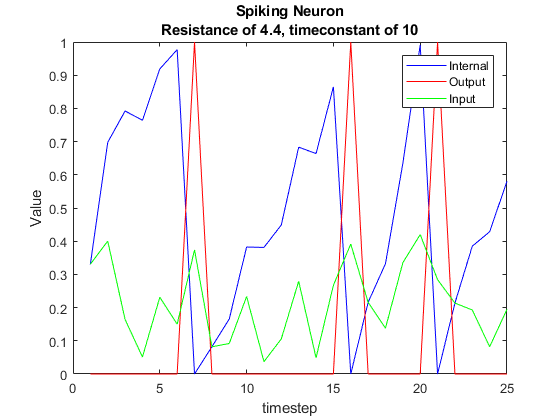
\includegraphics[width=\textwidth]{Images/fast.png}
        \caption{The neuron model using double resistance, and random input with a mean of 0.5.}
        \label{fig:implementation_test}
    \end{subfigure}
    \caption{Tests of the neuron model.(a) shows the ideal potential curve followed by a spike. (b) shows how the potential curve caused by a randomized input can be used in place of the ideal curve to get the same frequency of the spike. (c) shows how doubling the resistance parameter does not double the fireing rate of the neuron.}
    \label{fig:implementation_test}
\end{figure}

If one instead changes the parameters so that the resistance is twice of what it was in the baseline, and sets the input to a random number between zero and one each timestep, the result, as seen in figure \ref{fig:fast}, the neuron fires three times in the same timestep, showing how the resistance is not proportional to the fire rate of the neuron.

\section{Propagation}

In a functional Liquid State Machine, the activation of a neuron in the hidden layer will spread to nearby neurons like ripples in a pond. In order to test this, one can activate a single neuron and observe this behavior through the activation of the connected neurons. One way of performing this observation is by setting the neuron parameters in such a way that a single received pulse is enough to cause an activation, and then activating a single neuron in the reservoir. The expected behavior is a cascade effect where each activation will activate several other neurons, eventually activating each connected neuron in the reservoir.

By visualizing the activity of the network through repeated activations, this is easy to test. In figure \ref{fig:implementation_test}, it is clear that a single reservoir neuron is activated after the first timestep, and that after ten timesteps all connected neurons have been activated. In this figure it is also clear that three adjacent neurons, which is the number of connections each neuron have, are activated in the second timestep, as is expected from a functional Liquid State Machine.

\begin{figure}
    \centering
    \begin{subfigure}[b]{0.225\textwidth}
        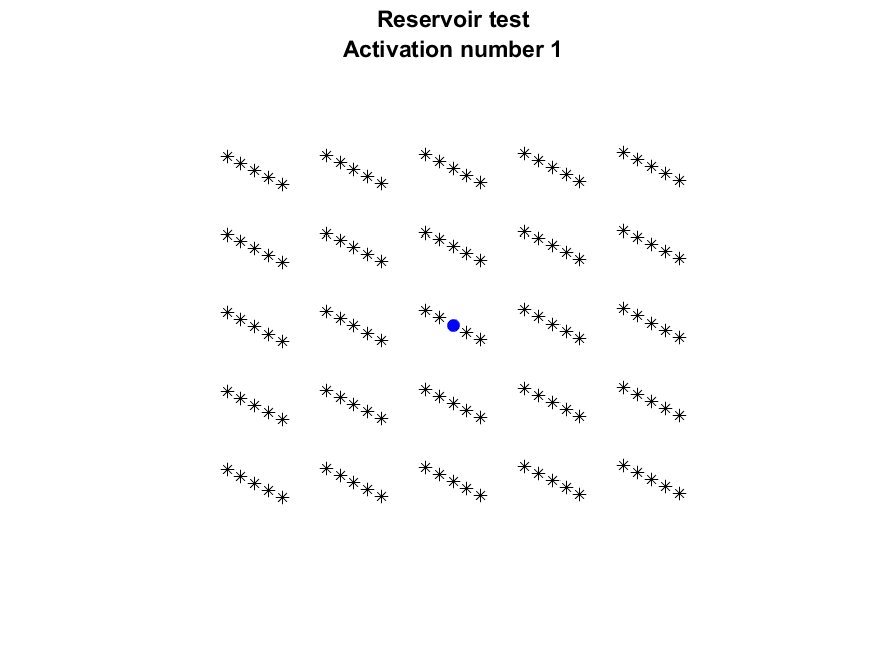
\includegraphics[width=\textwidth]{Images/Reservoir_test_Activation_number_1.png}
        \caption{The test network after a single timestep.}
    \end{subfigure}
    \begin{subfigure}[b]{0.225\textwidth}
        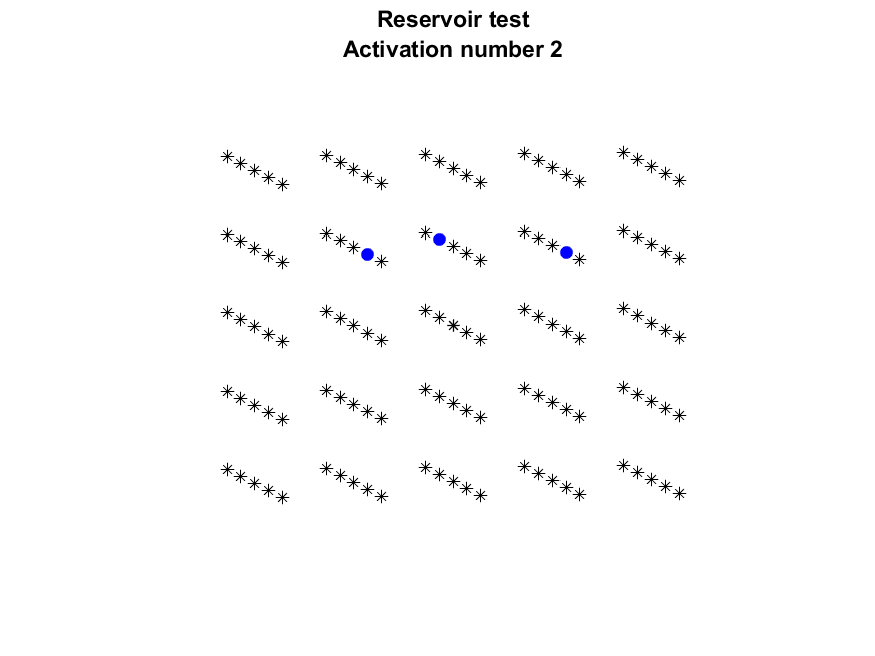
\includegraphics[width=\textwidth]{Images/Reservoir_test_Activation_number_2.png}
        \caption{The test network after two timesteps.}
    \end{subfigure}
    \begin{subfigure}[b]{0.225\textwidth}
        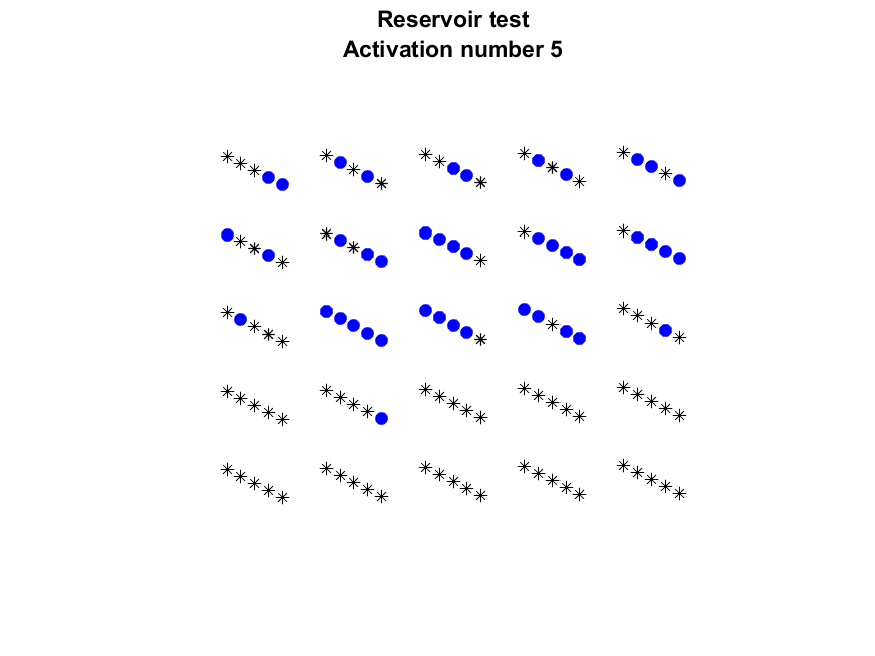
\includegraphics[width=\textwidth]{Images/Reservoir_test_Activation_number_5.png}
        \caption{The test network after five timesteps.}
    \end{subfigure}
     \begin{subfigure}[b]{0.225\textwidth}
        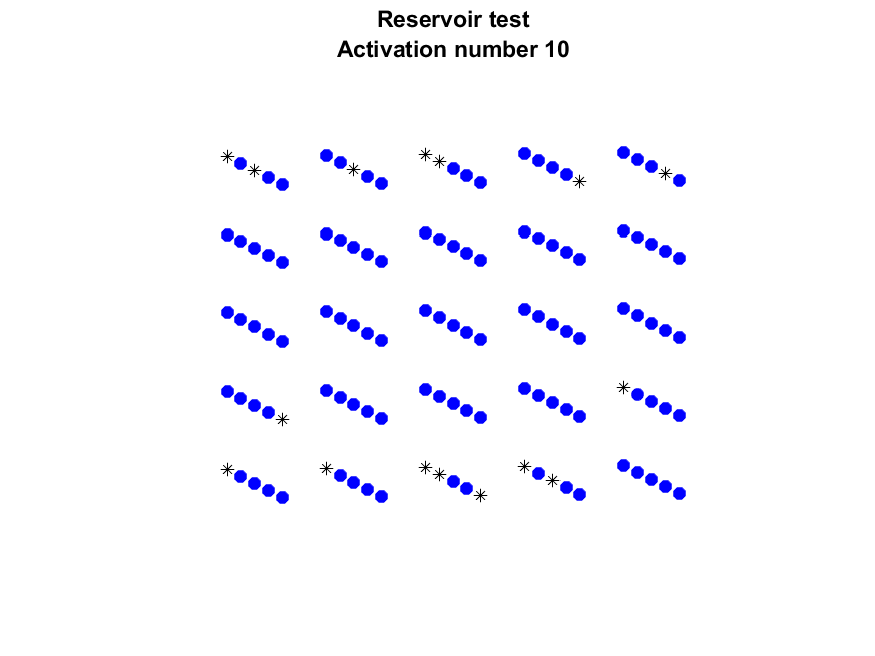
\includegraphics[width=\textwidth]{Images/Reservoir_test_Activation_number_10.png}
        \caption{The test network after ten timesteps.}
    \end{subfigure}
    \caption{Test of the propagation of the network. Every neuron has three synapses which are adjacent to it, and each spike will activate all three synases. After the first timestep, only the selected neuron is active. In the second timetep, it has spiked and is therefore inactive while the three neurons it has synapses to are active. After five timesteps a large proportion of the neurons are active, and after ten all connected neurons are active.}
    \label{fig:implementation_test}
\end{figure}

\section{Reservoir parameters}

The reservoir parameters are as important as the 

\section{Training}